%%% Version 2.1b %%%

\section{Logical Viewpoint}

\subsection{Overview}

Describes the system’s functional elements, their responsibilities, interfaces, and primary interactions. A Functional view is the cornerstone of most ADs and is often the first part of the description that stakeholders try to read. It drives the shape of other system structures such as the information structure, concurrency structure, deployment structure, and so on. It also has a significant impact on the system’s quality properties such as its ability to change, its ability to be secured, and its run-time performance. 

\subsection{Concerns and stakeholders}

\subsubsection{Concerns} 

\begin{itemize}
\item Functional capabilities. 
\item External interfaces.
\item Internal structure.
\item Functional design philosophy.
\end{itemize}

\subsubsection{Stakeholders}
\begin{itemize}
\item All stakeholders.
\end{itemize}

\subsection{Model}

\begin{itemize}
\item Functional structure model.
\end{itemize}

\subsection{Known issues with view}

\begin{itemize}
\item Poorly defined interfaces.
\item Poorly understood responsibilities. 
\item Infrastructure modeled as functional elements.
\item Overloaded view.
\item Diagrams without element definitions. 
\item Difficulty in reconciling the needs of multiple stakeholders.
\item Wrong level of detail.
\item `God’ elements
\item Too many dependencies.
\end{itemize}

\FloatBarrier

\begin{figure}[h!]
\centering
\caption{Logical Model}
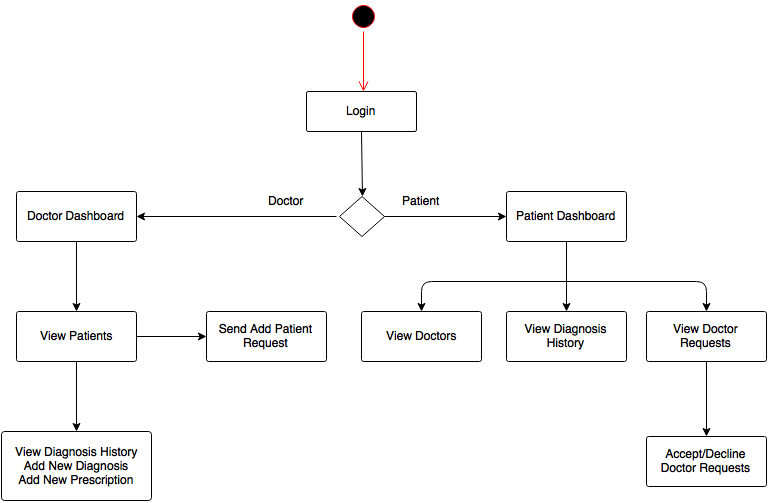
\includegraphics[width=16cm]{Logical.png}
\label{Basic Micro-services architecture pattern}
\end{figure}

\FloatBarrier

\section{Development Viewpoint}

\subsection{Overview}

Describes the architecture that supports the software development process. Development views communicate the aspects of the architecture of interest to those stakeholders involved in building, testing, maintaining, and enhancing the system.

\subsection{Concerns and stakeholders}

\subsubsection{Concerns}

\begin{itemize}
\item Module organization.
\item Common processing.
\item Standardization of design.
\item Standardization of testing.
\item Instrumentation.
\item Code-line organization.
\end{itemize}

\subsubsection{Stakeholders}

\begin{itemize}
\item Production engineers, software developers and testers.
\end{itemize}

\subsection{Model}

\begin{itemize}
\item Module structure models.
\item Common design models.
\item Code-line models.
\end{itemize}

\subsection{Known issues with view}

\begin{itemize}
\item Too much detail.
\item Overburdening the AD.
\item Uneven focus. 
\item Lack of developer focus.
\item Lack of precision.
\item Problems with the specified environment.
\end{itemize}

\FloatBarrier

\begin{figure}[h!]
\centering
\caption{Deployment Model}
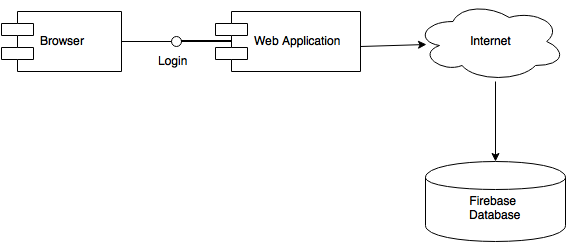
\includegraphics[width=16cm]{Deployment.png}
\label{Basic Micro-services architecture pattern}
\end{figure}

\FloatBarrier

\section{Physical Viewpoint}

\subsection{Overview}

Describes the environment into which the system will be deployed, including capturing the dependencies the system has on its run-time environment. This view captures the hardware environment that your system needs (primarily the processing nodes, network interconnections, and disk storage facilities required), the technical environment requirements for each element, and the mapping of the software elements to the run-time environment that will execute them. 

\subsection{Concerns and stakeholders}

\subsubsection{Concerns}

\begin{itemize}
\item Run-time platform required.
\item Specification and quantity of hardware or hosting required.
\item Third-party software requirements.
\item Technology compatibility.
\item Network requirements.
\item Network capacity required.
\item Physical constraints.
\end{itemize}

\subsubsection{Stakeholders}

\begin{itemize}
\item System administrators, developers, testers, communicators, and assessors.
\end{itemize}

\subsection{Model}

\begin{itemize}
\item Run-time platform models.
\item Network models.
\item Technology dependency models.
\item Inter-model relationships.
\end{itemize}

\subsection{Known issues with view}

\begin{itemize}
\item Unclear or inaccurate dependencies.
\item Unproven technology.
\item Unsuitable or missing service-level agreements.
\item Lack of specialist technical knowledge.
\item Late consideration of the deployment environment.
\item Ignoring inter-site complexities.
\item Inappropriate headroom provision.
\item Not specifying a disaster recovery environment.
\end{itemize}

\FloatBarrier

\begin{figure}[h!]
\centering
\caption{Physical Model}
\includegraphics[width=12cm]{Physical_model.png}
\label{Basic Micro-services architecture pattern}
\end{figure}

\FloatBarrier

\section{Process Viewpoint}

\subsection{Overview}

Describes how the system will be operated, administered, and supported when it is running in its production environment. For all but the simplest systems, installing, managing, and operating the system is a significant task that must be considered and planned at design time. The aim of the Operational viewpoint is to identify system-wide strategies for addressing the operational concerns of the system’s stakeholders and to identify solutions that address these.

\subsection{Concerns and stakeholders}

\subsubsection{Concerns}

\begin{itemize}
\item Installation and upgrade.
\item Functional migration. 
\item Data migration.
\item Operational monitoring and control.
\item Alerting.
\item Configuration management.
\item Performance monitoring.
\item Support.
\item Backup and restore.
\item Operation in third-party environments.
\end{itemize}

\subsubsection{Stakeholders}

\begin{itemize}
\item System administrators, developers, testers, communicators, and assessors.
\end{itemize}

\subsection{Model}

\begin{itemize}
\item Installation models.
\item Migration models.
\item Configuration management models. 
\item Administration models.
\item Support models.
\end{itemize}

\subsection{Known issues with view}

\begin{itemize}
\item Lack of engagement with the operational staff.
\item Lack of back-out planning.
\item Lack of migration planning.
\item Insufficient migration window.
\item Missing management tools.
\item Production environment constraints.
\item Lack of integration into the production environment 
\item Inadequate backup models.
\item Unsuitable alerting.
\end{itemize}

\FloatBarrier

\begin{figure}[h!]
\centering
\caption{Process Model}
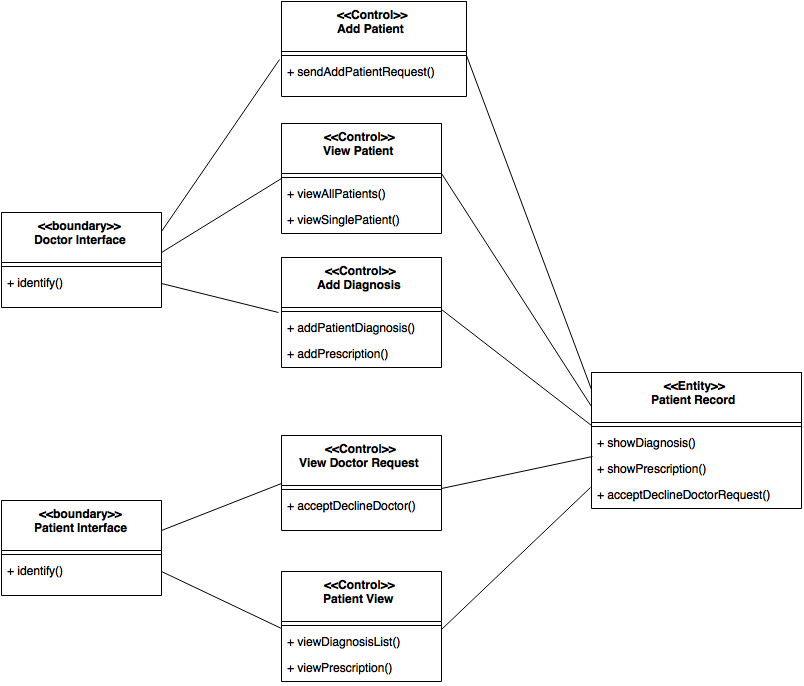
\includegraphics[width=16cm]{Process.png}
\label{Basic Micro-services architecture pattern}
\end{figure}

\FloatBarrier